\documentclass[a4paper, twoside, 11pt, openright]{article}
\usepackage[utf8]{inputenc}
\usepackage{polski}
\usepackage{float}
\usepackage[T1]{fontenc}
\usepackage{url}

\raggedbottom

\usepackage[left=3.0cm, right=2.0cm, top=2.5cm, bottom=2.5cm]{geometry}

% PERSONAL data about the thesis
\newcommand{\myTitle}{Metodyka porównania algorytmów prognozy do wspomagania decyzji giełdowych}
\newcommand{\myName}{Nikodem Wiśniewski}
\newcommand{\myNumber}{260907}
\newcommand{\myThesisType}{Praca dyplomowa magisterska}
\newcommand{\myCourse}{Informatyka}
\newcommand{\myProf}{dr hab. inż. Jerzy Balicki, profesor PW}
\newcommand{\myFaculty}{Wydział Matematyki i Nauk Informacyjnych}
\newcommand{\myUni}{Politechnika Warszawska}
\newcommand{\myLocation}{Warszawa}
\newcommand{\myYear}{2019}
\newcommand{\myKeywords}{}
\newcommand{\myKeywordsPL}{}



% DOCUMENT settings


\usepackage{graphicx}
\usepackage{multirow}
\usepackage{indentfirst}
\usepackage{wrapfig}
\usepackage[font=footnotesize, % equivalent to 9 pt font
			labelfont=bf, 
			justification=justified, 
			singlelinecheck=false]{caption} 
%\usepackage[justification=centering]{subcaption} % two images side by side captions
\usepackage{tabularx, booktabs} % pretty LaTeX tables
\usepackage{siunitx} % units SI e.g. \SI{10}{\kilogram\per\meter\square}
\usepackage{mathtools} % amsmath, symbols such as brackets, arrows, equation numbering only for referrenced eqs.
%\usepackage[parfill]{parskip} % spacing between paragraphs instead of indent
%\parfillskip 0pt plus 0.75\textwidth % get rid of widows at the end of paragraphs
\frenchspacing % for "Polish" spaces after the sentence
\usepackage{polski} % Polish rules of hyphenation
\usepackage{dashrule} % for dotted lines in declarations page
\usepackage{emptypage} % removes headers on empty pages
\usepackage{fancyhdr} % header and footer settings
\usepackage{subfigure}
\usepackage{cleveref}


\pagestyle{fancy}
\fancyhf{}
\newcommand{\fncyfront}{%
	\fancyhead[RO]{}
	\fancyfoot[RO]{}
	\fancyhead[LE]{}
	\fancyfoot[LE]{}
	\fancyhead[RE,LO]{}
	\fancyfoot[C]{}
	\renewcommand{\headrulewidth}{0pt}}
\newcommand{\fncymain}{%
	\fancyhead[RO]{{\footnotesize \rightmark}}
	\fancyfoot[RO]{\thepage}
	\fancyhead[LE]{{\footnotesize \leftmark}}
	\fancyfoot[LE]{\thepage}
	\fancyfoot[C]{}
	\renewcommand{\headrulewidth}{0.3pt}}
	
\renewcommand*{\tablename}{Tabela} 
	
\newcolumntype{P}[1]{>{\centering\arraybackslash}p{#1}}
\newcolumntype{M}[1]{>{\centering\arraybackslash}m{#1}}



% FONT settings
\usepackage[T1]{fontenc}

%\renewcommand{\familydefault}{\sfdefault} % change font to sans serif
\usepackage{amsfonts} % mathematical fonts
\usepackage{inconsolata} % monospaced font in urls and \texttt
%\usepackage{url}
%\urlstyle{same}

% DEBUG
\usepackage{lipsum}
\usepackage{etoolbox} % removes page number in table of contents
\patchcmd{\chapter}{plain}{empty}{}{}


\begin{document}
\fncyfront
%*******************************************************
% Titlepage
%*******************************************************
\begin{titlepage}
\begingroup
\begin{center}		
			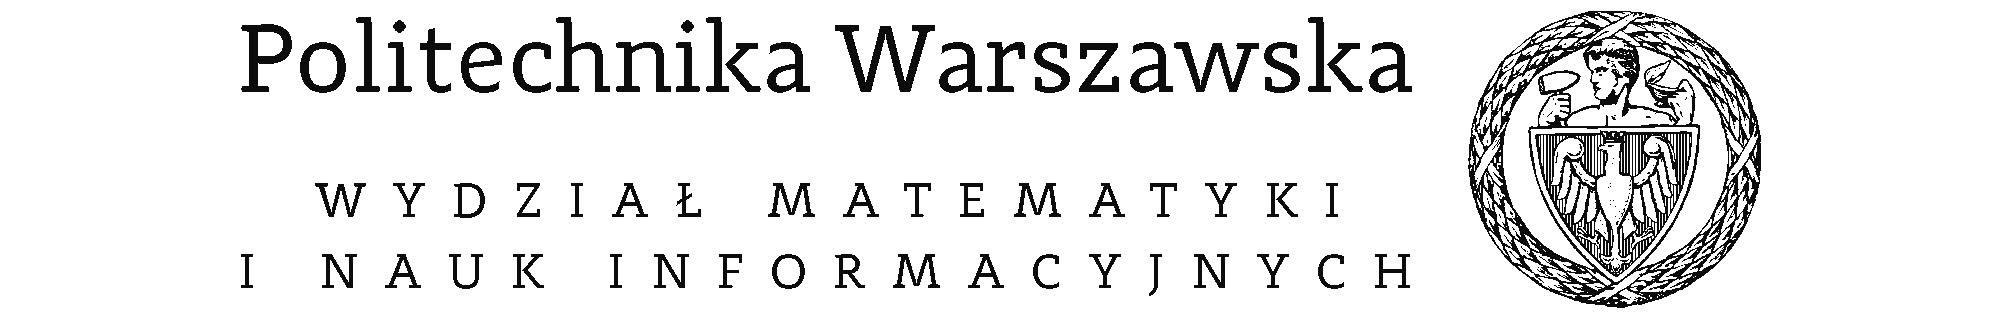
\includegraphics[width=1.0\textwidth]{img/pw_header}
			
			\vspace{1.0cm}
			\fontsize{24}{30}\selectfont\myThesisType
			\fontsize{12}{14}\selectfont
			
			\vspace{0.5cm}
			na kierunku \myCourse \\
			\vspace{1cm}
			{\fontsize{14}{18}\selectfont \myTitle} \\ 
			
			\vspace{1.5cm}
			\fontsize{21}{25}\selectfont \myName \\
			\fontsize{12}{14}\selectfont
			Numer albumu \myNumber \\

			\vspace{6.5cm}
			promotor \\
			\myProf \\
			\vspace{0.5cm}
			\vfill 
			Warszawa, \myYear
        \vfill                      
\end{center}
\endgroup
\end{titlepage}

\cleardoublepage

\begingroup
\fontsize{12pt}{14.4pt}\selectfont


\begin{abstract}
	Głównym celem pracy było opracowanie oraz porównanie modeli predykcyjnych pomagających w podejmowaniu decyzji maklerowi giełdowemu.

\bigskip

	\noindent \textbf{Słowa kluczowe:} giełda, predykcja, klasyfikacja, sieci neuronowe
\end{abstract}

\cleardoublepage


\hfill
\begin{table}[b]
\centering
\begin{tabular}[t]{ccc}
............................................. & \hspace*{100pt} & .............................................\\
podpis promotora & \hspace*{100pt} & podpis autora
\end{tabular}
\end{table}

\fncymain



\cleardoublepage

\tableofcontents

\cleardoublepage

\section{Modele prognozy na giełdzie oraz kryteria ich oceny}

Celem tej pracy jest opracowanie, ocena i porównanie różnych modeli predykcji cen akcji na giełdzie papierów wartościowych.

\subsection{Charakterystyka giełdy}

Giełda z definicji jest miejscem wymiany towarów przez sprzedawców i kupców. Giełdy można podzielić na giełdy towarowe, pieniężne lub usługowe. Wymiany na tradycyjnych giełdach przebiegają przede wszystkim podczas sesji, które są organizowane w określonych dniach i godzinach. Najpopularniejszym rodzajem giełd są giełdy pieniężne, a w szczególności giełdy papierów wartościowych. Największymi giełdami papierów wartościowych są \textit{NYSE (New York Stock Exchange)}\cite{nyse}, \textit{NASDAQ}\cite{nasdaq} oraz \textit{JPX (Japan Exchange Group)}\cite{jpx}. Na każdej z tych giełd w dniach, w których prowadzone są sesje, dochodzi do transakcji opiewających na łączną kwotę rzędu miliardów dolarów amerykańskich.

\bigskip

 Jednym z wymienianych na giełdzie towarów są akcje różnorodnych spółek. Każda spółka, która jest obecna na giełdzie ma przypisany do siebie symbol giełdowy (\textit{ticker}). Symbol giełdowy jest skrótowym kodem do identyfikowania spółek na określonej giełdzie (przykładowe symbole: \textit{GOOGL}, \textit{MSFT}, \textit{AMZN}). Podczas każdej sesji dokonywane są transakcje milionów akcji, których cena regulowana jest przez wolny rynek. Wynikiem tego jest duża zmienność cen i nieprzewidywalność akcji. Jest ona spowodowana między innymi: spekulacjami inwestorów, upublicznianiem informacji o konkretnej spółce (np. raportów finansowych) lub wydarzeniami na arenie politycznej (np. ustawy wpływające na działalność spólek z konkretnego sektora).


\subsection{Dane giełdowe}

Przed przystąpieniem do wyboru modeli należy zastanowić się nad danymi jakie będą służyć do ich uczenia. Wybór odpowiednich cech, analiza zebranych informacji oraz przetworzenie ich, wykracza poza zakres uczenia maszynowego tworząc własną dziedzinę zwaną inżynierią i analizą danych. Odpowiedni dobór i obróbka danych wejściowych często daje większe korzyści niż dopracowywanie modeli przewidujących i optymalizacja ich parametrów. 

\subsubsection{Dane podstawowe}

Podstawowymi (dziennymi) danymi wynikającymi bezpośrednio z funkcjonowania giełdy są:

\begin{itemize}
\item{Data}
\item{Cena zamknięcia} - cena akcji pod koniec dnia
\item{Cena otwarcia} - cena akcji na początku dnia
\item{Liczba akcji w obrocie danego dnia}
\item{Najniższa cena akcji danego dnia}
\item{Najwyższa cena akcji danego dnia}
\end{itemize}

 Przy korzystaniu z wartości cen akcji należy również uwzględnić podział akcji(tak zwany \textit{split}). Gdy jakaś spółka decyduje się na podział swoich akcji oznacza to, że każda z akcji dzieli się na dwie akcje o cenie wynoszącej połowę pierwotnej ceny. Taki zabieg pozwala na zmniejszenie ceny pojedynczej akcji dzięki czemu może stać się ona dostępna dla większej liczby inwestorów. 
 
\bigskip

Powyższe dane nie wnoszą jednak zbyt wiele informacji ponieważ są odzwierciedleniem powstałego obrotu akcji na giełdzie, a nie jego przyczyną. W związku z dużą losowością ruchów giełdowych, są niewystarczające aby skutecznie przewidzieć zmiany cen akcji. Zawodowi maklerzy do podejmowania swoich decyzji wspomagają się dodatkowo dwoma technikami: \textbf{analizą fundamentalną} oraz \textbf{analizą techniczną}.

\subsubsection{Analiza fundamentalna \cite{fundamentalanalysis}}

Analiza fundamentalna spółek jest analizą kondycji ekonomicznej spółek w zestawieniu z wartością ich akcji. Ten rodzaj analizy ma odpowiedzieć na pytanie czy cena akcji konkretnej spółki odpowiada jej sytuacji na rynku. Przy takim badaniu spółki brane jest pod uwagę wiele różnych czynników, takich jak:
\begin{itemize}
\item{analiza finansowa spółki}
\item{analiza sektorowa}
\item{analiza makroekonomiczna}
\item{analiza ogólnej sytuacji spółki}
\end{itemize}

Ten rodzaj badania spółek jest niezwykle czasochłonny i często wymaga eksperckiej wiedzy w dziedzinie finansów. Dodatkowo analiza fundamentalna wymaga posiadania danych, publicznych aczkolwiek czasami ciężko dostępnych, o spółkach i sektorach, w których się znajdują. Analizę fundamentalną stosuje się w szczególności przy inwestycjach długoterminowych (np. kilka miesięcy).

Najsłynniejszym analitykiem technicznym świata jest \textit{Warren Buffet} prezes amerykańskiego holdingu \textit{Berkshire Hathaway \cite{berkeshire}}. 


%Analiza fundamentalna ze względu na swoją długoterminową naturę (raporty finansowe spółek publikowane kwartalnie) jest mało istotna przy dziennych predykcjach giełdowych. Z tego względu zostanie ona pominięta w tej pracy.

\subsubsection{Analiza techniczna \cite{technicalanalysis}}

Analiza techniczna jest zbiorem technik mających na celu wspomaganie inwestora w podejmowaniu decyzji na podstawie historycznych danych giełdowych. Analiza ta bada zachowania rynku oraz poszukuje trendów np. poprzez analizę kształtów wykresów giełdowych. Szczególnie istotne są liczne wskaźniki techniczne oraz narzędzia analizy statystycznej.
Najpopularniejsze wskaźniki techniczne obejmują:
\begin{itemize}
\item{\textbf{SMA}} - średnia krocząca. Jest to średnia cen z kilku ostatnich dni (np. 3, 7, 14, 30),
\item{\textbf{EMA}} - wykładnicza średnia krocząca. Jest to wykładnicza średnia cen z kilku ostatnich dni (np. 3, 7, 14, 30),
\item{\textbf{MACD}} -  miara zbieżności i rozbieżności średnich ruchomych,
\item{\textbf{RSI}} -  wskaźnik siły względnej określający siłę trendu,
\item{\textbf{oscylator stochastyczny}} -  wskaźnik momentum i siły trendu.
\end{itemize}

\subsubsection{Źródło danych}

W pracy zostało wykorzystane darmowe źródło danych giełdowych \textit{Alpha Vantage} \cite{alphavantage}. Jest to API pozwalające na pobranie historycznych danych giełdowych dla konkretnej spółki poprzez podanie odpowiedniego symbolu giełdowego. Dostępne są zarówno podstawowe dane giełdowe jak i wskaźniki analizy technicznej. 

\subsection{Predykcja}

Na rysunku \ref{alphabet_history} widoczne są zmiany cen akcji spółki \textit{Alphabet Inc.} w latach 2004-2018. Analizując ten wykres z łatwością można wskazać daty, w których opłacalnym było zainwestowanie w akcje, aby następnie je sprzedać w póżniejszym terminie by osiągnąć zysk. Niestety stwierdzenie czy wartość akcji w przyszłości spadnie, czy wzrośnie, nie jest tak trywialne jak odczytywanie danych historycznych. Przewidywanie przyszłych cen akcji jest głównym zajęciem zarówno inwestorów indywidualnych jak i instytucjonalnych. Skuteczne odgadywanie przyszłych wzrostów lub spadków cen pozwoliłoby na osiąganie ponadprzeciętnych zysków i unikanie strat. O trudności tego zadania mogą świadczyć takie teorie jak \textit{hipoteza błądzenia losowego} czy też \textit{hipoteza rynku efektywnego}. Zgodnie z \textit{hipotezą błądzenia losowego} \cite{randwalk}, krótkoterminowo, ceny akcji zmieniają się według nieprzewidywalnych schematów. Zmiany minutowe cen akcji są więc dużo trudniejsze do przewidzenia niż zmiany dobowe. \textit{Hipoteza rynku efektywnego} \cite{efficientmarket} opiera się na założeniu iż ceny obecne na giełdzie całkowicie odwzorowują wszystkie dostępne informacje na rynku. Oznacza to, że próby wyprzedzenia innych inwestorów na podstawie szybkiej reakcji na pojawiające się informacje nie będą skuteczne. Obie te hipotezy mają zarówno swoich zwolenników jak i krytyków.

\begin{figure}[H]
\centering 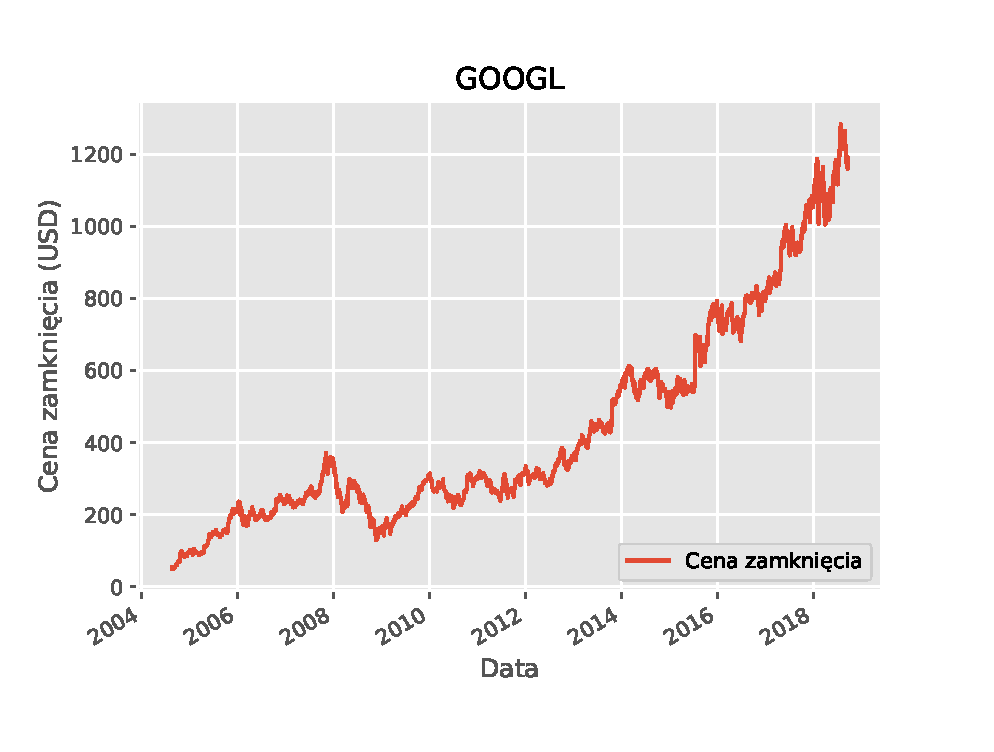
\includegraphics[scale=0.9]{img/linear_regression/l_r_stock_data}
\caption{Wykres cen akcji spółki \textit{Alphabet Inc} (opracowanie własne)}
\label{alphabet_history}
\end{figure}

Rysunek \ref{alphabet_history} ilustruje fakt, że ceny zamknięcia akcji tworzą szereg czasowy. Dotyczy to także pozostałych charakterystyk akcji, takich jak cena otwarcia, liczba akcji w obrocie danego dnia, najniższa cena akcji czy najwyższa cena akcji danego dnia. Fakt ten ma istotny wpływ na sposób używania i przetwarzania danych giełdowych.

\subsubsection{Zakres prognozy}

Przed przystąpieniem do konstruowania modeli predykcyjnych należy zdefiniować co tak naprawdę warto przewidywać, każda akcja ma bowiem kilka atrybutów. Najbardziej pożytecznym parametrem akcji, którego wykorzystanie daje inwestorowi największe szanse na zysk jest \textbf{cena zamknięcia}. Znajomość ceny zamknięcia z kolejnego dnia daje inwestorowi cały czas trwania sesji giełdowej na podjęcie skutecznych decyzji inwestycyjnych. Jest to najczęściej wybierany parametr akcji przy przewidywaniu ceny. Przykładem parametru, który nie jest istotny jest liczba akcji w obrocie z kolejnych dni, ta liczba sama w sobie nie niesie informacji o spadku lub wzroście cen.

\bigskip

Po wybraniu celu prognozy należy również określić jej przedział czasowy. Ceny na giełdzie można przewidywać dla dowolnego przedziału czasu. Może to być zarówno okres jednej minuty jak i kilku miesięcy. Przy gwarancji doskonałych prognoz, im większa częstotliwość dokładnego przewidywania ceny tym lepiej. Wynika to z tego iż inwestor może szybciej reagować na zachodzące zmiany i w większym stopniu wykorzystywać pozyskaną wiedzę zwiększając zyski. Z drugiej strony opierając się na \textit{hipotezie błądzenia losowego} można zauważyć, że zmiany w małych przedziałach czasowych są dużo bardziej zaburzone przez losowe wahania ceny. To z kolei sprawia iż krótkoterminowe ruchy cen mogą okazać się nie do przewidzenia. W celu utrzymania kompromisu pomiędzy użytecznością modelu, a jego odpornością na losowość giełdy, za okres predykcji został wybrany \textbf{jeden dzień}.
 
\subsubsection{Prognozowanie - regresja czy klasyfikacja?}

Do tematu prognozowania cen akcji można podejść na dwa sposoby:
\begin{itemize}
\item{\textbf{dokładny}, przewidywanie konkretnych wartości cen akcji,}
\item{\textbf{binarny}, predykcja wzrostu lub spadku ceny - tak zwana predykcja trendu.}
\end{itemize}

Potencjalnie korzystniejszym podejściem jest przewidywanie dokładnych cen akcji, gdyż jest to dokładniejsze aproksymowanie ceny. Jednakże z perspektywy inwestora istotniejszym od dokładnych wartości ceny są trendy. To właśnie różnice w cenach akcji pozwalają zarobić na ich obrocie. Wobec tego zamiast przewidywania dokładnej ceny zamknięcia warto przewidywać wzrosty oraz spadki cen. W przeciwieństwie do danych ciągłych, wyjściowe dane dyskretne  dają jasny sygnał o działaniach jakie należy podjąć aby zarobić. Z tego powodu jako podstawowe wyjście z modeli predykcyjnych wybrany został \textbf{trend binarny}.

\bigskip

Ze względu na to jak przebiega obrót akcjami, binarne przewidywanie z dnia na dzień może jednak okazać się niedostosowane do rzeczywistości. Akcje kupuje i sprzedaje się za pomocą domu maklerskiego, który pobiera prowizje za każdą transakcję. Obecnie najniższe prowizje na polskim rynku są na poziomie $0,19\%$ za transakcję. Pojedyncza operacja dająca zarobić na przewidzianej cenie wymaga kupienia, a następnie sprzedania akcji, wobec czego łączna prowizja wyniesie przy zaokrągleniu $0,4\%$. Wszystkie wahania cen poniżej tej wartości są teoretycznie bez znaczenia dla inwestora, ponieważ nie da się na nich zarobić. W związku z powyższym wnioskowaniem należy zastosować model dyskretny, będący rozwinięciem modelu binarnego o dodatkową klasę - klasę utrzymania ceny w pewnych ramach. Wyszczególnione są wówczas trzy klasy:
\begin{itemize}
\item spadek ceny poniżej $0,4\%$
\item wzrost ceny powyżej $0,4\%$
\item utrzymanie zmiany ceny w przedziale $(-0,4; 0,4)\%$
\end{itemize}

Dla potwierdzenia zasadności takiego modelu, należy upewnić się że dzienne wahania cen na giełdzie są wystarczające. Na rysunku \ref{l_r_pct_change_last_30} można zaobserwować, iż zmiany w kursie często przekraczają $0,4\%$ w związku z czym transakcje przynoszące zysk można wykonywać regularnie. Ten wniosek potwierdza zasadność takiej konstrukcji modeli. W związku z większym stopniem złożoności takiej klasyfikacji, może okazać się iż dane wejściowe nie pozwalają na odseparowanie tych trzech klas. 

%TODO dodać paski -0.4%   +0.4% do wykresu
\begin{figure}[H]
\centering 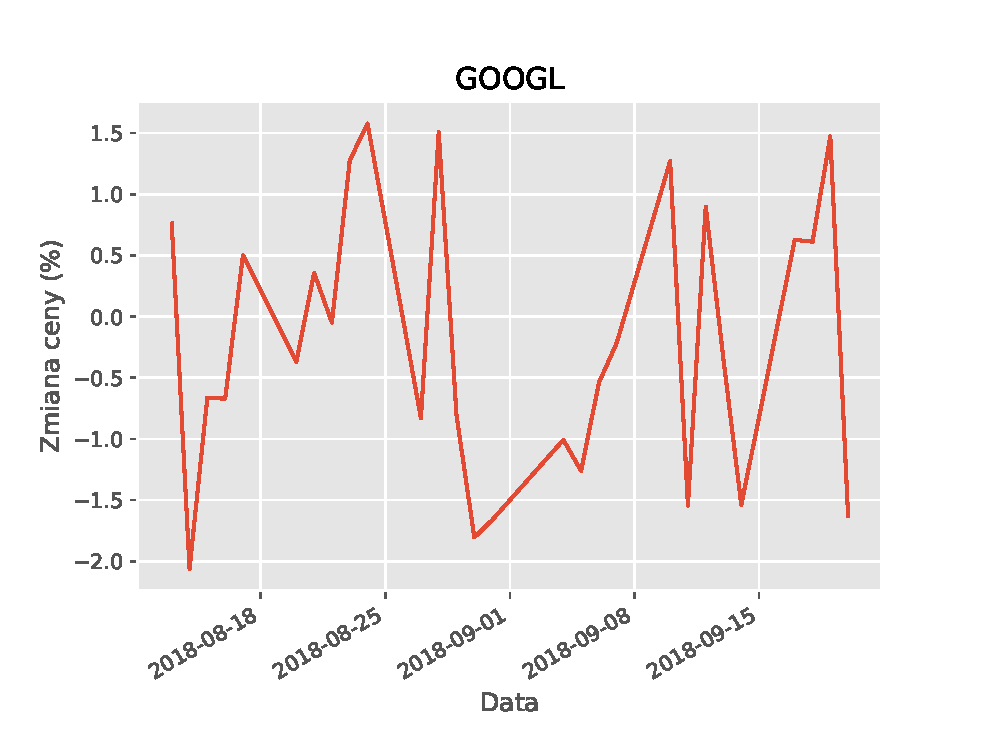
\includegraphics[scale=0.9]{img/linear_regression/l_r_pct_change_last_30}
\caption{Dzeinna zmiana ceny akcji spółki \textit{GOOGL} z 30 dni (opracowanie własne)}
\label{l_r_pct_change_last_30}
\end{figure}


\subsection{Metodyka konstruowania modeli}

Ponieważ zagadnienie przewidywania giełdy jest nietrywialne ze względu na losowe wahania wpływające na ceny akcji, do stworzenia każdego z modeli do predykcji, należy rozważyć wykorzystanie zróżnicowanych założeń:
	
\begin{itemize}
\item{\textbf{Prognozowanie dokładne/dyskretne} }
\item{\textbf{Liczba dni}, z których prognozowana jest wartość.}
\item{\textbf{Dobór danych wejściowych}, selekcja wartości wejściowych}
\item{\textbf{Dobór spółek uczących i testujących}}
\end{itemize}


\subsubsection{Perspektywa prognozy}

Model przewidujący może na wyjściu zwrócić predykcje z więcej niż jednego dnia sesji giełdowej. Należy uważać jednak na nakładanie się błędów predykcji i uważnie dobierać parametr przewidywanej liczby dni. Na przykład, jeżeli prognozowana jest wartość na dwa dni do przodu, to wówczas trzeci prognozowany dzień będzie oparty na prognozie z poprzedniego dnia. W związku z czym dojdzie złączenia się błędu i zwiększenia zaburzenia wyników.

\subsubsection{Liczba dni historycznych}

Wektor wejściowy do modelu może składać się z wielu parametrów giełdowych z jednego wybranego dnia z przeszłości. Możliwa jest również konkatenacja takich wektorów z kilku poprzednich dni dająca modelowi wgląd w kształtowanie się ruchu cen na przestrzeni czasu. Taki zabieg daje modelom większą ilość informacji. Dobranie większej ilości informacji może zarówno pogorszyć jak i polepszyć wyniki modelu. Jest to więc jeden z parametrów, który należy rozważyć.

\subsubsection{Selekcja cech}

Według niektórych badań wolumen obrotów akcji nie jest skorelowany w żaden sposób z jej ceną. Modele mogą więc wykazywać lepsze wyniki przy mniejszej lub większej liczbie wejściowych parametrów. Niektóre parametry mogą okazać się zbędne lub wręcz mogą osłabiać przewidywanie wartości.

\subsubsection{Dobór spółek}

Modele oceniane na podstawie danych poszczególnych spółek mogą dawać w skrajnych przypadkach zafałszowane wyniki. Wiele spółek wykazuje wysoką korelację cen akcji między sobą. W celu uniknięcia pułapki przetrenowania, do uczenia i testowania użyte zostały dane spółek o niskiej korelacji i różnych trendach wzrostu/spadku.

\subsection{Kryteria oceny modeli predykcji}

Podczas oceny modelu wzięto pod uwagę różne kryteria mierzenia dokładności nauczonych klasyfikatorów.
\begin{itemize}
\item procent prawidłowych klasyfikacji
\item pole pod krzywą ROC
\item częściowy indeks Gini
%\item statystyka H
\item współczynnik Briera
\item statystyka Kołomogrowa-Smirnova
\end{itemize}

\subsubsection{Macierz błędu}

W przypadku klasyfikacji dwuklasowej na klasy A i B każdą predykcję można przypisać do jednej z 4 grup:
\begin{itemize}
\item True Positive (TP) - gdy przewidziano klasę A dla etykiety A
\item False Negative (FN) - gdy przewidziano klasę B dla etykiety A
\item False Positive (FP) - gdy przewidziano klasę A dla etykiety B
\item True Negative (TN) - gdy przewidziano klasę B dla etykiety B
\end{itemize}

%TODO dodać schemat macierzy błedu

Graficzną reprezentację podziału klasyfikacji na powyższe kategorie nazywamy \textit{macierzą błędu}. Zastosowanie miar opartych o tablicę błędów dla problemów z większą liczbą klas wymaga dodatkowych kroków. W celu policzenia wartości TP, FN, FP i TN należy wyróżnić konkretną klasę, a pozostałe klasy należy zagregować w sztuczną klasę przeciwną. W ten sposób należy wyliczyć konkretną miarę tyle razy ile jest klas. Ostatecznym krokiem w celu uzyskania jednolitej oceny modelu jest na przykład wyliczenie średniej ważonej z wyników dla każdej z klas.


\subsubsection{Procent prawidłowych klasyfikacji}

Jednym z najprostszych sposobów do oceny dokładności klasyfikatorów jest określenie procentu prawidłowych przypisań przykładu do klasy. Metoda ta potrafi dawać złudzenie zadowalających wyników, w których występują duże różnice w licznościach poszczególnych klas. Rozważmy dla takiego zadania naiwny model przypisujący do każdego postawionego przykładu klasę, której liczność jest największa. Wówczas wyniki procentowe prawidłowej klasyfikacji będą wprost proporcjonalne do różnicy w liczności klasy największej w stosunku do innych klas. W większości przypadków pomimo dobrego wyniku taki model będzie uznany za bezużyteczny. Wobec tego tę miarę jakości należy stosować wraz z innymi miarami, które nie są podatne na tego typu zaburzenia.

\subsubsection{Pole AUC pod krzywą ROC \cite{roc}}

Krzywa ROC (ang. receiver operating characteristic) jest narzędziem, która opisuje dokładność klasyfikatora za pomocą oceny jego czułości i precyzji. Precyzją modelu nazywa się stosunek $\frac{TP}{TP+FP}$, zaś czułość jest oznaczona przez $\frac{TP}{TP+FN}$.

\bigskip

Zdefiniujmy wartości \textit{True Positive Rate (TPR)} oraz \textit{False\ Positive\ Rate (FPR)}:

$$ TPR = \frac{TP}{TP+FN}\ \ \ \ \ \ \ \ FPR = \frac{FP}{FP+TN} $$

Klasyfikatory w większości przypadków nie zwracają dokładnego wyniku przypisania przykładu do klasy. Zazwyczaj wynikiem klasyfikacji jest liczba rzeczywista z przedziału $[0, 1]$, którą można identyfikować jako prawdopodobieństwo. Można przyjąć że jeżeli klasyfikator zwróci $0$ oznacza to przypisanie do klasy A, zaś $1$ oznacza przypisanie do klasy B. Dla wartości z zakresu $(0, 1)$ przypisuje się pewną wartość progową rozgraniczającą obie klasy. Dla tego progu mniejsze od niego wartości przypisujemy do klasy A, zaś resztę do klasy B. Intuicyjnie jest to zazwyczaj połowa przedziału czyli $0.5$.

Krzywa ROC jest graficzną reprezentacją skuteczności modelu klasyfikacyjnego. Jest ona skonstruowana poprzez wykreślenie stosunku $TPR$ do $FPR$ dla różnych progów rozgraniczających klasy. Na rysunku \ref{roc} widać przykładowe krzywe ROC dla klasyfikatorów różnej jakości.


%source: https://towardsdatascience.com/understanding-auc-roc-curve-68b2303cc9c5
\begin{figure}[H]%
\centering
\subfigure[Krzywa ROC dla modelu, który nie jest w stanie rozdzielić klas]{%
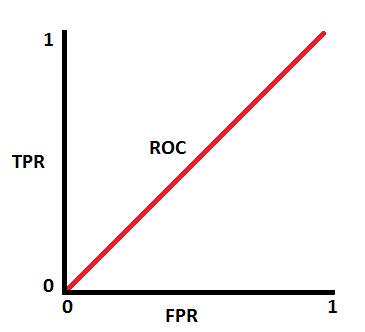
\includegraphics[scale=0.55]{img/roc_1.png}}%
\qquad
\subfigure[Krzywa ROC przykładowego klasyfikatora]{%
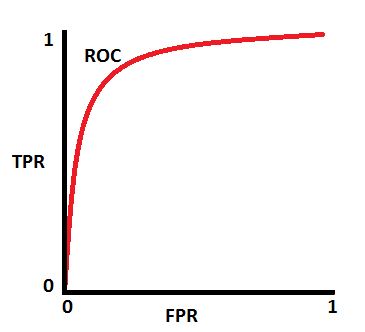
\includegraphics[scale=0.55]{img/roc_2.png}}%
\qquad
\subfigure[Krzywa ROC dla modelu idealnego]{%
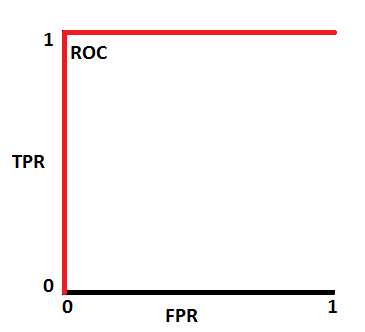
\includegraphics[scale=0.55]{img/roc_3.png}}%
\caption{Przykładowe krzywe ROC \cite{roccurves} }% (źródło: https://towardsdatascience.com/understanding-auc-roc-curve-68b2303cc9c5).}
\label{roc}
\end{figure}


Porównanie różnych klasyfikatorów za pomocą krzywej ROC odbywa się poprzez porównanie pola pod krzywymi. Im większe pole pod krzywą ROC dla danego klasyfikatora tym lepsza jest jego jakość. Pole pod krzywą dla modelu idealnego wynosi $1$, zaś dla modelu losowego $0.5$. Warto zauważyć że dla wartości pola poniżej 0.5  korzystnym zabiegiem jest zamiana przedziałów dla klas.


\subsubsection{Częściowy indeks Gini} %TODO bibliografia

%TODO dodać wykres z indeksem GINI

Częściowy indeks Gini jest innym sposobem na analizę jakości modelu predykcyjnego za pomocą krzywej ROC. Otrzymuje się go poprzez wyliczenie pola powierzchni pomiędzy krzywą ROC dla modelu predykcyjnego, a krzywą ROC dla modelu losowego, w stosunku do pola powierzchni między krzywą ROC modelu idealnego, a krzywą ROC modelu losowego. Dla modelu losowego wynosi 0, zaś dla modelu idealnego wartość indeksu wynosi 1. W ten sposób otrzymana wartość indeksu Gini może być interpretowana jako procent idealności modelu.

\subsubsection{F1} %TODO bibliografia

Metryka F1 jest średnią harmoniczną metryk czułości i precyzji (wyrażona wzorem $F1=2*\frac{precyzja*czulosc}{precyzja+czulosc}$). Metryka ta jest dobrym narzędziem pozwalającym określić za pomocą jednej wartości jakość modelu, biorąc pod uwagę precyzję jak i czułość modelu. Osiąga ona w najlepszym przypadku wartość 1, zaś w najgorszym wartość 0. 

%\subsubsection{Miara H \cite{hmeasure}}

%TODO dodać wykres z krzyżującymi się krzywymi ROC dla różnych modeli

%Miary oparte o krzywą ROC mimo wielu zalet mają również wady \cite{roccritique}. Gdy pole pod krzywą pierwszego klasyfikatora jest mniejsze od pola pod krzywą drugiego klasyfikatora, można wywnioskować iż drugi klasyfikator jest lepszy. Bywa jednak że krzywe ROC dla tych dwóch modeli się krzyżują, a pierwszy model pomimo mniejszego pola powierzchni pod krzywą, ma lepsze właściwości dla znacznej większości progów używanych do rozdzielenia klas. Należy również wziąć pod uwagę iż analizy porównawczej modeli klasyfikujących często dokonuje się dla małych, stopniowych optymalizacji parametrów. Powoduje to zazwyczaj małe różnice w nakreślonych krzywych ROC, które mogą się krzyżować. W związku z powyższym miary oparte o tą krzywą nie dają dobrego porównania modeli w takim scenariuszu.
 
%\bigskip

%Przy ocenie modeli warto również wziąć pod uwagę czy błąd predykcji z grupy \textit{FP} jest równoważna wynikowi z \textit{FN}. Niech dany będzie problem klasyfikacji binarnej kursu giełdy z klasami \textit{wzrost (positive)} oraz \textit{spadek (negative)}. W przypadku gdy wynik zaklasyfikowany zostanie do grupy \textit{FP}, wówczas makler giełdowy korzystający z tego klasyfikatora zainwestuje pieniądze pomimo spadającego kursu. Oznacza to najgorszą możliwą decyzję narażającą użytkownika modelu na straty. W drugim przypadku gdy wynik zostanie przypisany do grupy \textit{FN}, makler zostanie fałszywie ostrzeżony przed spadkiem kursu. Wówczas sprzedaż akcji może jedynie ograniczyć jego zyski, zakładając że wcześniej zainwestował poprawnie (przed wzrostem cen akcji). Z powyższego można wywnioskować, iż ocena powinna być surowsza dla klasyfikacji przykładów w grupie \textit{FP}.
 
%\bigskip
%https://cran.r-project.org/web/packages/hmeasure/vignettes/hmeasure.pdf rozdział 2.6 

%\textit{Miara H} jest miarą oceny modeli klasyfikujących zaproponowaną przez D.J.Hand, która została opracowana jako alternatywa dla miar opartych o krzywą ROC. Metodyka ta daje możliwość wzięcia pod uwagę wiedzy eksperckiej na temat kosztu przypisania wyniku do złej klasy (\textit{FP} lub \textit{FN}). Niech $c \in [0,1]$ będzie kosztem przypisania elementu do grupy FP, zaś $1-c$ kosztem przypisania elementu do grupy FN. Niech $t$ będzie progiem rozdzielającym klasy. Całkowity koszt klasyfikacji to:

%$$ \pi_{0}=\frac{TP+FN}{n} \ \ \ \ \ \ \ \ \  \pi_{1}=\frac{TN+FP}{n} $$
%$$ L(c,t) = 2(c\pi_{0}FPR(t)+(1-c)\pi_{1}(1-TPR(t))$$



%Warto zauważyć że $L(\frac{1}{2}, t)$ odpowiada mierzeniu procentu prawidłowych klasyfikacji.

%Wartość funkcji $L(c,t)$ należy minimalizować w celu uzyskania jak najlepszej klasyfikacji. Wobec czego można zdefiniować $MLW(c)=L(c,T_c)$ gdzie $T_c$ jest  takim progiem klasyfikacji dla danego $c$, który minimalizuje $L(c,t)$ ($T_c = argmin_tL(c,t)$). Funkcja $MLW(c)$ oceniająca konkretny model klasyfikujący jest zależna od tylko jednej zmiennej. W praktyce jednak ciężko jest oczekiwać od użytkownika tej miary, doboru optymalnej wartości zmiennej $c$. Wobec tego zaproponowane zostało używanie rozkładu $w(c)$ zamiast konretnej zmiennej $c$. 

%$$ L_w=\int_{c}L(c, T_c)w(c)dc $$

%Miarę H zdefiniowana jest wzorem:

%$$ H = 1-\frac{L_w}{L_w^{max}} $$

%gdzie $L_w^{max}$ jest maksymalną wartością funkcji $L_w$, służącą do znormalizowania wyniku. Im większa wartość $H$ tym lepsza ocena klasyfikatora.
%https://link.springer.com/content/pdf/10.1007%2Fs10994-009-5119-5.pdf L_w^{max} zdefiniowane na stronie 116

\subsubsection{Współczynnik Briera \cite{brier}}

Współczynnik Briera (ang. Brier score) jest metodą oceny modeli klasyfikujących opisana wzorem:

$$	BS=\frac{1}{N} \sum_{t=1}^{N} \sum_{i=1}^{R}(f_{ti}-o_{ti})^2 $$

\begin{itemize}
\item $N$ to liczba predykcji,
\item $R$  to liczba możliwych klas
\item $f_{ti}$ to prawdopodobieństwo, które wyznaczył klasyfikator, przypisania przykładu $t$ do klasy $i$,
\item $o_{ti}$ to rzeczywiste przypisanie przykładu do danej klasy (0 gdy przykład nie jest tej klasy, oraz 1 gdy przykład należy do tej klasy).
\end{itemize}

W związku z powyższą definicją, miara ta może zostać wykorzystana w przypadku modeli, które na swoim wyjściu zwracają prawdopodobieństwo przypisania przykładu do każdej z klas. Wobec tego nie każdy model można ocenić tą metryką. Istotnym spostrzeżeniem jest fakt iż w przeciwieństwie do innych metryk, współczynnik Briera modelu idealnego wynosi $0$, zaś im gorszy model tym większy współczynnik.


%TODO źródło do poniższego
\subsubsection{Statystyka Kołmogorowa-Smirnova}

Statystyka Kołmogorowa-Smirnova (ang. Kolmogrow-Smirnov Test) pozwala ocenić jakość klasyfikatora binarnego na podstawie stopnia separacji rozkładu dwóch klas. Ocena dokonywana jest przez zmierzenie maksymalnej odległości między wkyresami dystrybuant rozkładu jednej i drugiej klasy. Niech $F(x)$ to dystrybuanta rozkład klasy 1, zaś $G(x)$ to dystrybuanta rozkładu klasy 2. Wówczas statystyka Kołmogorowa-Smirnova opisana jest wzorem:

$$D_{n,m}=\sup_x|F(x)-G(x)|$$

Metryka ta daje wartość 100 dla modelu idealnego, zaś 0 dla modelu losowego.

\subsection{Wnioski i uwagi}

Porównanie modeli klasyfikujących jest zadaniem trywialnym tylko dla specyficznych problemów. W tych przypadkach można się oprzeć o procent prawidłowych klasyfikacji jako jedyną miarę jakości modeli. W bardziej złożonych przypadkach dochodzi do dysproporcji w rozmiarze klas, wówczas ta podstawowa miara zostaje w pewien sposób zafałszowana. Innym aspektem, który może być brany pod uwagę przy ocenie klasyfikatorów jest różnica w wadze błędu z grupy \textit{FP}, względem błędu z grupy \textit{FN}. Te problemy należy rozwiązywać poprzez używanie wielu miar do porównywania modeli. Używanie wielu metryk może być przydatne w szczególności gdy dwa modele mają podobne wartości w jednej z miar.

\bigskip

W zagadnieniu predykcji giełdowych sprowadzonym do klasyfikacji, można posłużyć się procentem prawidłowych klasyfikacji jako podstawową miarą porównawczą. Wynika to z faktu, iż dla większości spółek liczność klas się równoważy. Dla dokładniejszego porównania modeli warto jednak zastosować również inne metryki, które dadzą więcej wglądu w otrzymywane wyniki.
% Przy bardziej zaawansowanych badaniach należy uwzględnić przede wszystkim \textit{miarę H}, która bierze pod uwagę większy błąd fałszywego przypisywania predykcji do grupy wzrostów cen.

\newpage

\section{Wybrane algorytmy do prognozowania}

\subsection{Regresja za pomocą regresji liniowej}

Jedną z naiwnych metod przewidywania wartości funkcji jest regresja liniowa. Pierwszą próbą dla tego modelu było przewidzenie ceny zamknięcia z kolejnego dnia przy posiadaniu danych z dnia poprzedniego.

Z rysunku \ref{linear_regression_1} wynika iż prognozowane wartości pokrywają się z rzeczywistymi. Po obliczeniu błędu model daje nam dokładność na poziomie około  $99,934\%$. Wydaje się to być doskonałym wynikiem. Aby upewnić się o wartości modelu należy przyjrzeć się wykresowi z bliska.


\begin{figure}[H]%
\centering
\subfigure[Wykres rzeczywistych wartości]{%
\label{l_r_stock_data}
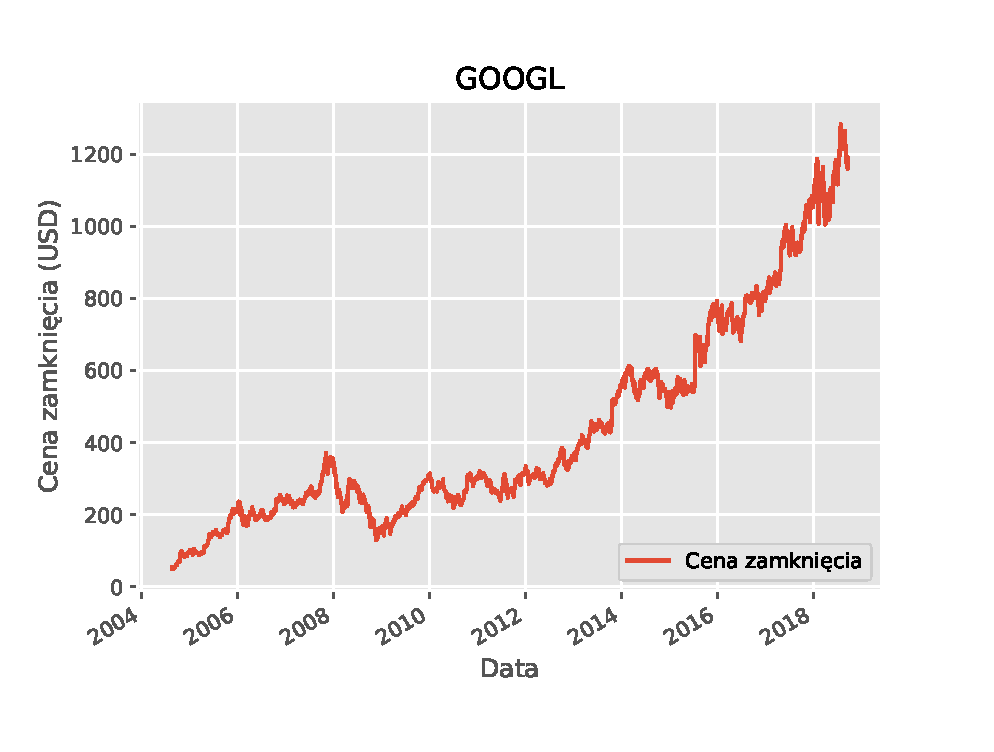
\includegraphics[scale=0.46]{img/linear_regression/l_r_stock_data}}%
\qquad
\subfigure[Wkyres rzeczywistych oraz przewidywanych wartości]{%
\label{l_r_1_day_full}
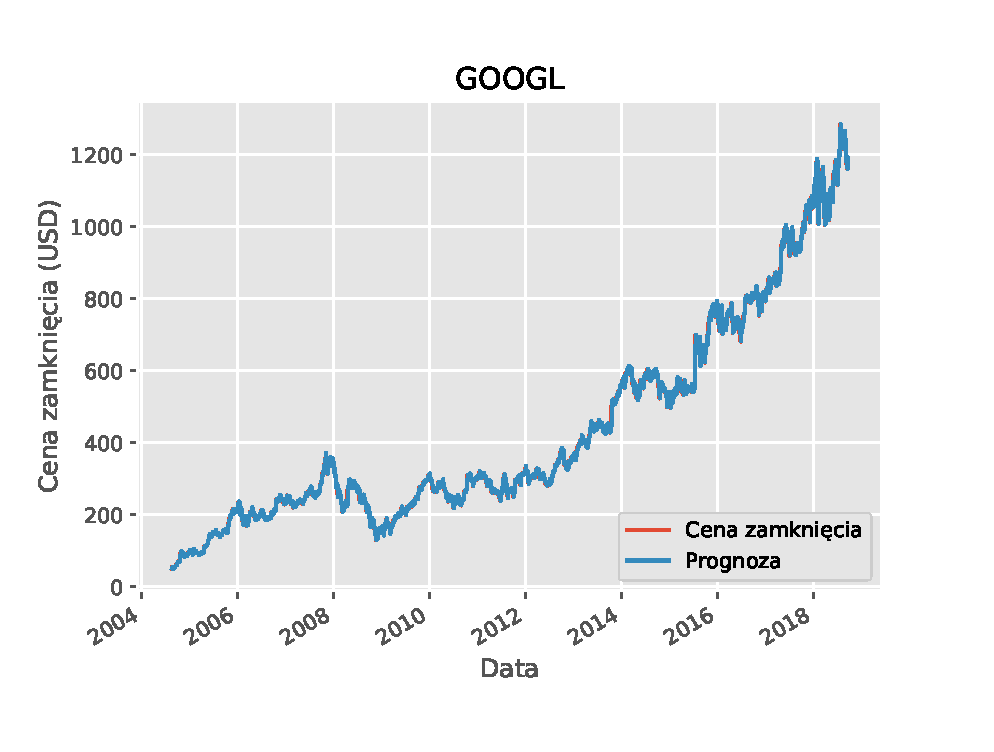
\includegraphics[scale=0.46]{img/linear_regression/l_r_1_day_full}}%
\caption{Wykres dla spółki \textit{GOOGL} (opracowanie własne)}
\label{linear_regression_1}
\end{figure}


Na rysunku \ref{l_r_1_day_last_30} widać że prognozowane wartości są w rzeczywistości delikatnie zniekształconym obrazem przeszłych notowań spółki. Dokładność na poziomie $~99\%$ została osiągnięta ze względu na małe wahania w cenie. Logicznie rzecz biorąc nie jest to dobra metoda przewidywania przyszłości. Gdy cena jest w lokalnym maksimum wówczas inwestor powinien sprzedać posiadane akcje, jednak model przewiduje dalsze wzrosty ceny i wprowadza inwestora w błąd. Analogiczna sytuacja dzieje się przy minimach lokalnych ceny akcji. 

\begin{figure}[H]
\centering 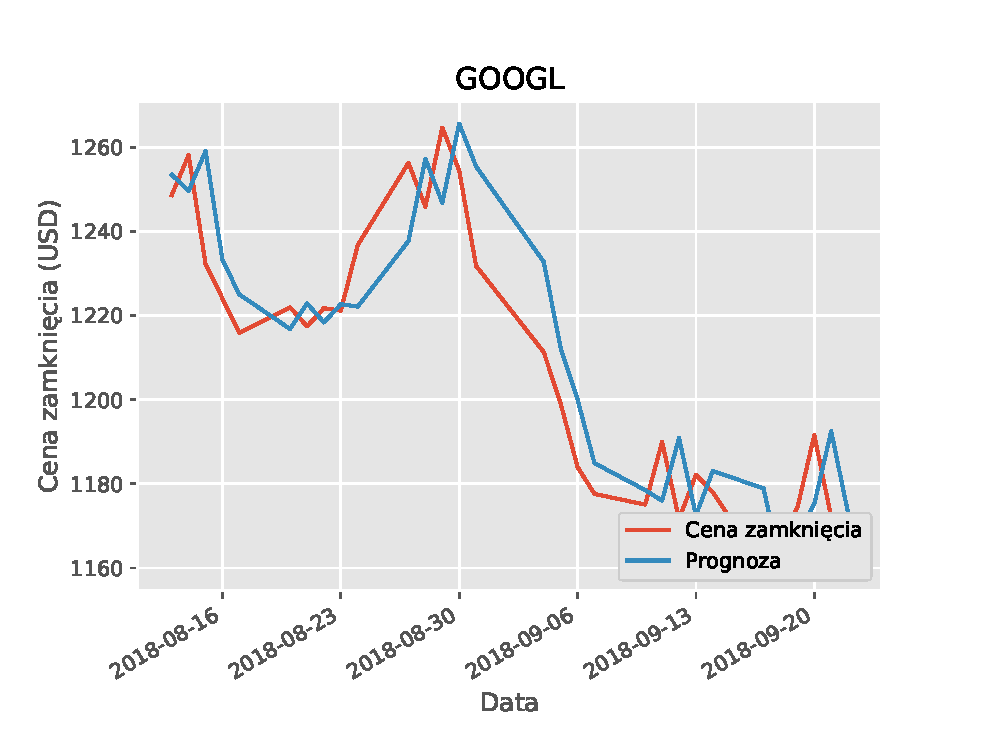
\includegraphics[scale=0.9]{img/linear_regression/l_r_1_day_last_30}
\caption{Wykres dla spólki \textit{GOOGL} z 30 dni (opracowanie własne)}
\label{l_r_1_day_last_30}
\end{figure}


\bigskip

Wobec powyższych obserwacji należy sprawdzić jakość tego modelu w metodą dyskretnej. Dla tych samych prognoz została przeprowadzona ocena dyskretna z progiem $\pm0,4\%$. Na rysunku \ref{l_r_discrete_score} widoczna są przewidywane oraz rzeczywiste wartości oceny dyskretnej. Ze względu na charakterystyke regresji liniowej, niemal wszystkie prognozy oscylują w granicach, które są nieznaczące dla inwestora. Ocena tą metodą dała wynik $0.257\%$ co udowadnia bezużyteczność tego modelu. Dla porównania model losowy z rozkładem jednostajnym dałby wynik na poziomie $0.(3)\%$.


\begin{figure}[H]
\centering 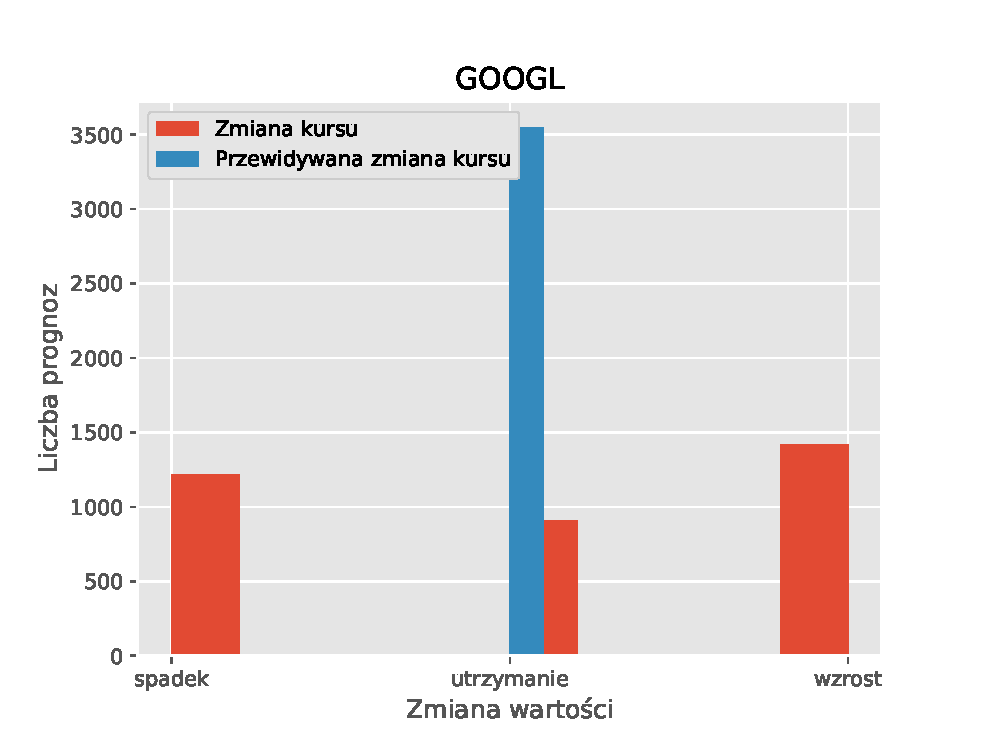
\includegraphics[scale=0.9]{img/linear_regression/l_r_discrete_score}
\caption{Histogram zmian cen akcji spółki \textit{GOOGL} (opracowanie własne)}
\label{l_r_discrete_score}
\end{figure}

\subsection{SVM \cite{svm}}

Maszyny wektorów podpierających (ang. support-vector machines) są zbiorem klasyfikatorów mających na celu wyznaczenie hiperpłaszczyzn rozdzielających klasy z zachowaniem maksymalnego marginesu rozdzielającego (rysunek \ref{wiki_svm}). W podstawowej wersji klasyfikatory SVM potrafią sktuecznie klasyfikować problemy separowalne liniowo.


\begin{figure}[H]
\centering 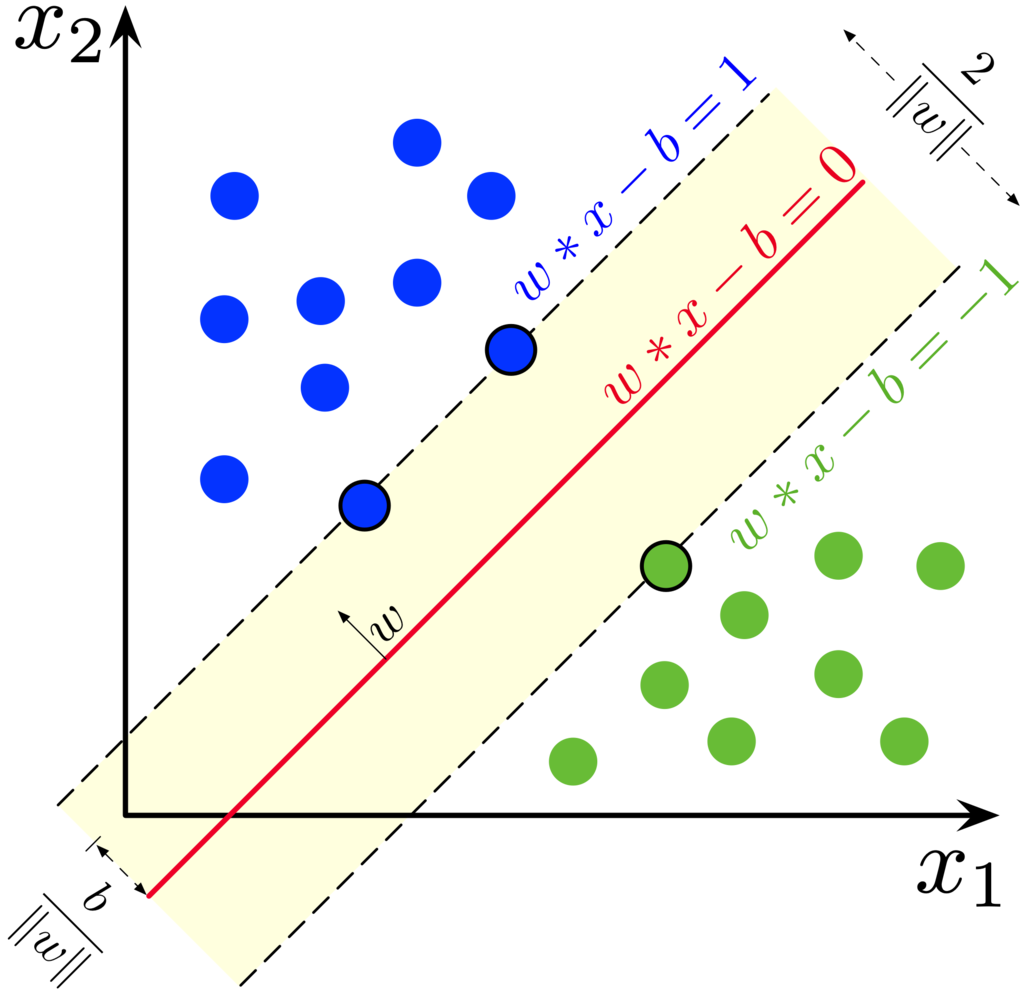
\includegraphics[scale=0.9]{img/svm.png}
\caption{Hiperpłaszczyzna rozdzielająca zbiór z maksymalnym marginesem \cite{wikisvm}}
\label{mlpnn}
\end{figure}

W celu używania maszyn wektorów nośnych do klasyfikacji problemów nieliniowych stosuje się przekształcanie przestrzeni zadania za pomocą funkcji jądrowych. Wprowadzają one dodatkowe wymiary do zadania, w których znalezienie hiperpłaszczyzny rozdzielającej klasy może okazać się prostsze (rysunek \ref{wiki_svm2}. Do najpopularniejszych funkcji jądrowych zalicza się funkcje: liniową (zachowującą wymiar zadania w niezmienionym stanie), wielomianową, radialną czy też sigmoidalną.


\begin{figure}[H]
\centering 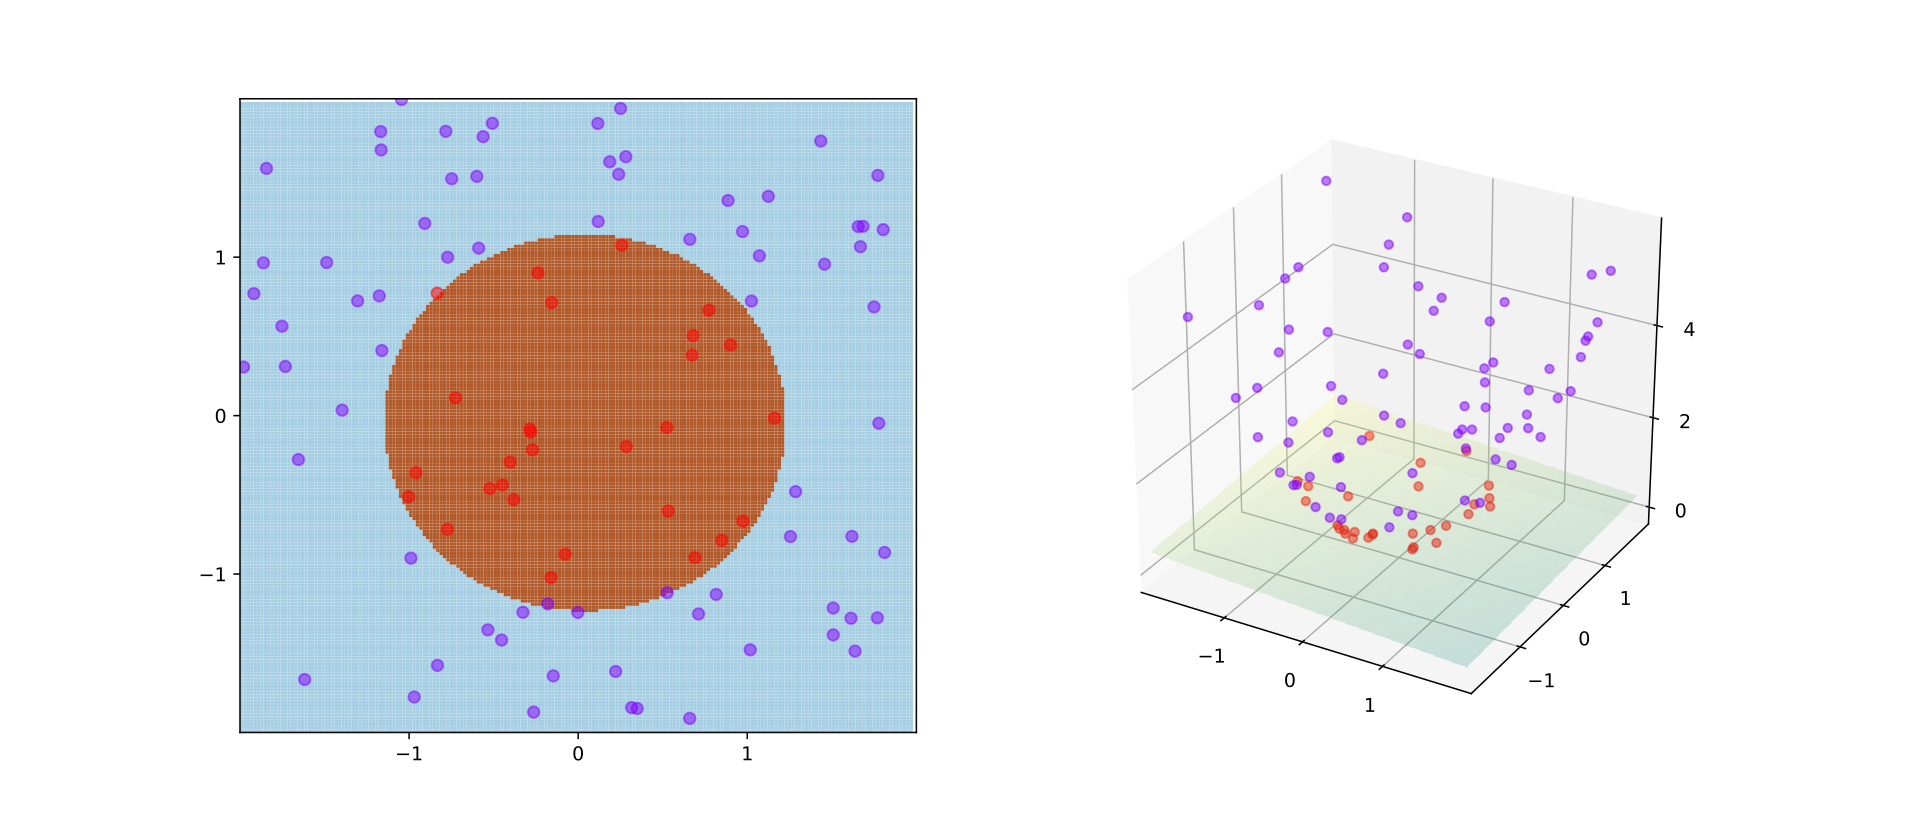
\includegraphics[scale=0.2]{img/svm2.png}
\caption{Ten sam problem zaprezentowany w dwóch oraz trzech wymiarach \cite{wikisvm}}
\label{wiki_svm2}
\end{figure}


\subsection{Sieci neuronowe \cite{neural-nets}}

Sieci neuronowe są zbiorem modeli matematycznych służących do realizacji obliczeń, bądź przetwarzania sygnałów. Inspirowane działaniem mózgu, swoją nazwę czerpią z upodobnienia struktury do naturalnych neuronów oraz łączących je synaps. Głównymi zastosowaniami sieci neuronowych są zadania regresji, klasyfikacji oraz generowania danych. 

\bigskip

Podstawowym elementem sieci neuronowej jest neuron, który na wejściu przyjmuje dane wejściowe, przetwarza i zwraca pojedynczy sygnał wyjściowy. Przetwarzanie sygnału przez neuron z polega zazwyczaj na zsumowaniu sygnałów dochodzących do niego, a następnie obliczenie wartości funkcji aktywacji. Uzyskana wartość z funkcji aktywacji jest przekazywana jako wyjście z neuronu (rysunek \ref{neural-net}). Funkcje aktywacji mogą wprowadzić element nieliniowy do modelu dzięki czemu sieci neuronowe mogą posłużyć do klasyfikacji zbiorów, które nie są separowalne liniowo. Dodatkowo połączenia między neuronami posiadają przypisaną wagę mającą bezpośredni wpływ na wartość sygnału przechodzącego między nimi.

\bigskip

Wiodącym schematem uczenia sieci neuronowych jest korzystanie z przykładów, z których każdy ma etykietę czyli oczekiwaną wartość wyjściową. Każdy z przykładów jest przetwarzany przez sieć neuronową, następnie przez zestawienie wartości wyjściowej sieci z etykietą (odpowiednią funkcją straty) można wyliczyć błąd sieci dla danego przykładu. Ostatnim krokiem jest poprawa wag w sieci neuronowej według wybranej metody propagacji wstecznej. Problem optymalizacji sieci neuronowej sprowadzany jest do problemu optymalizacji funkcji poprzez modyfikację wag na połączeniach między neuronami. Metoda ta zaliczana jest do nauczania z nauczycielem (ang. supervised learning). Najczęściej stosowanymi metodami optymalizacji są algorytmy spadku gradientowego. 

\bigskip

Przy wykorzystywaniu sieci neuronowych głównym problemem, z którym zmagają się naukowcy jest odpowiedni dobór parametrów i algorytmów. Spośród elementów wymagających odpowiedniego dobrania wymienić można następujące:
\begin{itemize}
\item liczba warstw sieci,
\item liczba neuronów w każdej z warstw ukrytych,
\item wykorzystane funkcje aktywacji,
\item algorytm optymalizacyjny,
\item funkcja straty.
\end{itemize}


\subsubsection{Sieci typu MLP \cite{mlp}}

Jednym z najprostszych przykładów sieci neuronowych jest perceptron wielowarstwowy (ang. multilayer perceptron). Taka sieć składa się z warstwy wejściowej, z dowolnej ilości warstw ukrytych oraz z warstwy wyjściowej. W tym rodzaju sieci neuronowych, sygnał wyjściowy dowolnego neuronu jest traktowany jako sygnał wejściowy każdego z neuronów z kolejnej warstwy (rysunek \ref{neural-net}). 

\bigskip

\begin{figure}[H]
\centering 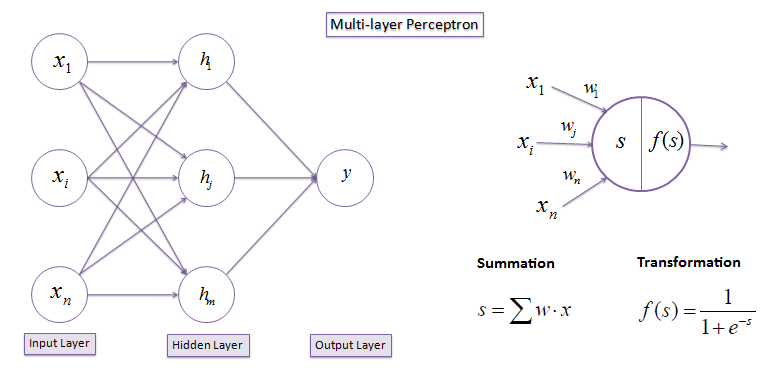
\includegraphics[scale=0.7]{img/nn.png}
\caption{Schemat sieci neuronowej typu MLP \cite{mlpnn}}
\label{neural-net}
\end{figure}

Najprostszą implementacja sieci do predykcji danych giełdowych jest sieć przyjmująca na wejściu wektor informacji o akcjach spółki z jednego dnia, zwracająca na wyjściu przewidywaną wartość ceny akcji następnego dnia. Perceptron wielowarstwowy można również zaprojektować tak, aby na wyjściu zwracał wynik klasyfikacji, czyli procentowy wynik przypisania danych wejściowych do każdej z możliwych klas. W tej pracy badane były sieci neuronowe klasyfikujące dane wejściowe według trzech klas: spadek wartości poniżej pewnego progu, utrzymanie wartości w ramach tego progu oraz wzrost wartości powyżej tego progu. 


\subsubsection{Sieci rekurencyjne}

W przeciwieństwie do sieci MLP, sieci rekurencyjne posiadają sprzężenia zwrotne sygnału wychodzącego z neuronów. Dzięki wtórnemu sygnałowi sieci te posiadają pewną pamięć przepływających sygnałów. Wpływem sygnału wtórnego na końcowy wynik można sterować za pomocą wag na połączeniach między odpowiednimi neuronami.

\subsubsection{Sieć typu LSTM \cite{lstm}}

Sieci LSTM (ang. Long Short Term Memory) są specjalnym rodzajem sieci rekurencyjnych, będących w stanie zapamiętywać długoterminowe zależności. Jak widać na rysunku \ref{lstm-net} sieć typu LSTM jest postaci łańcucha komórek. Każda komórka jest odpowiedzialna za zestawienie i przetworzenie sygnału wejściowego $x_t$ z sygnałem wychodzącym z poprzedniego modułu.

\begin{figure}[H]
\centering 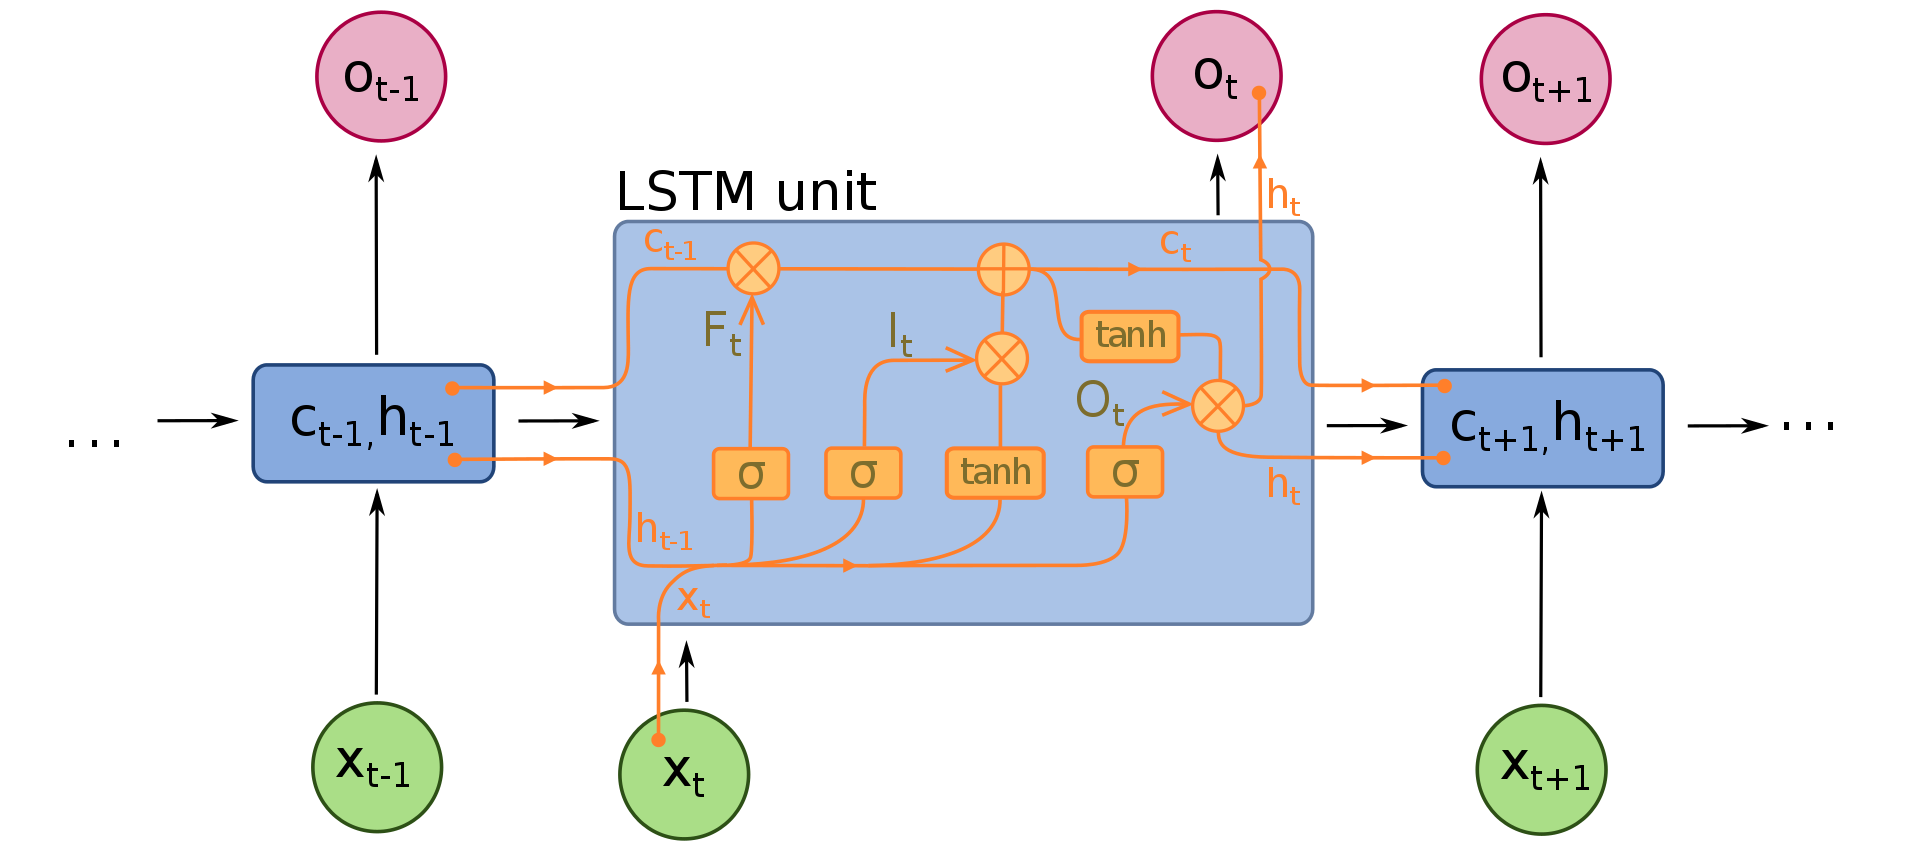
\includegraphics[scale=0.22]{img/lstm.png}
\caption{Schemat sieci neuronowej typu LSTM \cite{lstm-scheme}}
\label{lstm-net}
\end{figure}

Głównym elementem każdej komórki jest sygnał $c_{t-1}$ zmieniający się w $c_{t}$, który jest jej stanem. Pierwszym krokiem przy zmianie stanu komórki jest $F_t$ z funkcją sigmoidalną,tak zwana forget gate layer.  Odpowiada ona za zdecydowanie, jaka część sygnału zostanie odrzucona. Kolejnym elementem jest $i_t$, \textit{input gate layer}, która decyduje o tym jakie dane wejściowe zostaną użyte do zmiany stanu komórki. Ostatecznie warstwa $O_t$, \textit{output layer}, decyduje o tym jaka część sygnału powinna przejść do następnej komórki.

\bigskip

W ostatnich latach sieci tego rodzaju znajdują szerokie zastosowanie w takich dziedzinach jak rozpoznawanie mowy, tłumaczenia czy też opisywanie obrazów. Sieci LSTM mogą również być użyteczne w pracy z szeregami czasowymi, gdzie możliwe są zależności danych w czasie, tak jak na przykład na 
giełdzie. 

\subsection{Metody zespołowe}

Metody zespołowe (ang. ensemble methods) polegają na tworzeniu wielu klasyfikatorów o małej złożoności, które w odosobnieniu nie dają zadowalających wyników (często są niewiele lepsze od klasyfikatora losowego), a następnie łączenie ich w komitety. Wyniki komitetów mogą być interpretowane na wiele sposobów np. poprzez głosowanie gdzie każdy członek komitetu oddaje swój głos na konkretny wynik klasyfikacji. Okazuje się że w praktyce stosowanie tej metody często daje bardzo konkurencyjne wyniki w stosunku do stosowania pojedynczych złożonych modeli klasyfikacyjnych bądź regresyjnych.

\subsection{Random forest \cite{randforest}}

Las losowy (ang. \textit{random forest}) jest modelem opartym o drzewa decyzyjne służącym do klasyfikacji lub regresji. Drzewa decyzyjne są graficzną metodą wspomagania procesu decyzyjnego. W przypadku zagadnień uczenia maszynowego drzewa decyzyje najprościej zobrazować na przykładzie problemu klasyfikacji binarnej. Na rysnku \ref{wiki_dec_tree} przedstawione jest drzewo decyzyjne dla problemu predykcji losu pasażerów statku Titanic. Drzewo to oparte jest o trzy cechy: płeć, wiek oraz liczbę rodzeństwa oraz współmałżonków (\textit{sibsp}). 

\begin{figure}[H]
\centering 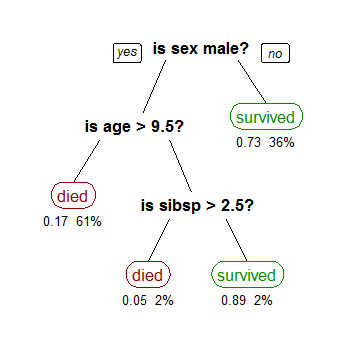
\includegraphics[scale=0.6]{img/decision_tree.png}
\caption{Drzewo decyzyjne dla problemu klasyfikacji losu pasażerów statku Titanic \cite{wikidecisiontree}}
\label{wiki_dec_tree}
\end{figure}

Dla złożonych zagadnień predykcji takich jak przewidywanie trendu giełdy, drzewa decyzyjne okazują się zbyt prostym modelem. Las losowy jest rozwinięciem koncepcji drzew decyzyjnych w zakresie metod zespołowych. Głównym założeniem jest stworzenie wielu drzew decyzyjnych i opieranie końcowego wyniku na podstawie poszczególnych wyników każdego z drzew. W celu wprowadzenia różnorodności podczas konstrukcji węzłów drzew, losowane są cechy spośród których będą dobrane cechy decyzyjne w danym węźle. Metoda ta zazwyczaj daje dużo lepsze efekty niż pojedyncze drzewa decyzyjne, oraz często pomaga w ograniczaniu zjawiska przeuczania (ang. overfitting).  

\subsubsection{Light GBM \cite{lgbm}}

\textit{Light GBM} jest algorytmem z rodziny \textit{gradient boosting decision trees}. Algorytmy te oparte są o zespół drzew decyzyjnych. W przeciwieństwie do metody \textit{lasu losowego} konstrukcja kolejnych drzew jest wykonywana w sposób sekwencyjny, oraz zależny od wyników poprzednich drzew. Dzięki takiemu zabiegowi, zespół drzew dąży do ulepszenia swoich wyników jako całości. Algorytm \textit{light GBM} przewyższa inne algorytmy ze swojej klasy takie jak \textit{XGBoost} dzięki innemu podejściu do tworzenia drzew. Podczas gdy większość algorytmów powiększa drzewa decyzyjne wgłąb (\textit{level-wise}  rysunek \ref{level-wise}), \textit{light GBM} powiększa drzewa decyzyjne ze względu na liście (\textit{leaf-wise} rysunek \ref{leaf-wise}). Ten zabieg wraz z innymi optymalizacjami sprawia, że algorytm ten osiąga porównywalne wyniki do innych algorytmów ze swojej klasy, przy dużym skrócenia czasu uczenia się. 


\begin{figure}[H]%
\centering
\subfigure[Konstrukcja drzewa algorytmu \textit{light GBM}]{%
\label{level-wise}
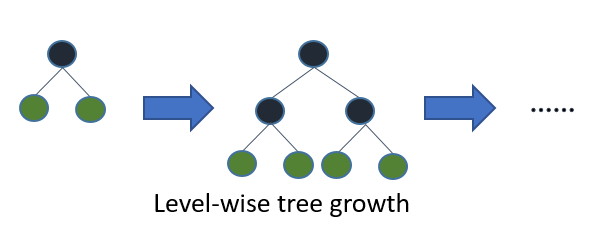
\includegraphics[scale=0.46]{img/lgbm-level-wise.png}}%
\qquad
\subfigure[Konstrukcja drzewa algorytmu \textit{light GBM}]{%
\label{leaf-wise}
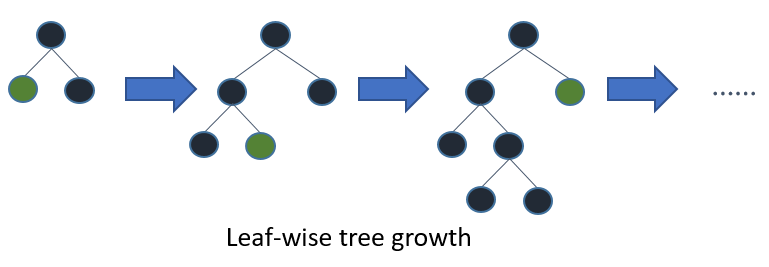
\includegraphics[scale=0.46]{img/lgbm-leaf-wise.png}}%
\caption{Porównanie konstrukcji drzew algorytmów z rodziny \textit{gradient boosting decision trees}}
\label{level-leaf-wise}
\end{figure}






%TODO \subsection{Wykorzystanie wykrywania sentymentu do poprawienia predykcji}

\subsection{Wnioski i uwagi}

Predykcja kursu cen na giełdzie jest zagadnieniem zaawansowanym pod względem trudności i złożoności danych. Z tego powodu w tej pracy zastosowane zostały różnorodne modele klasyfikacyjne zgodne z najnowszymi trendami w dziedzinie uczenia maszynowego. Użycie zarówno tradycyjnych modeli sieci neuronowych jak i nowoczesnych technik takich jak algorytm \textit{Light GBM} pozwoliło na obszerne badanie w zakresie poszukiwania najlepszego klasyfikatora.

\newpage

\section{Wspomaganie decyzji giełdowych}

\newpage

\section{Projekt aplikacji}

\newpage

\section{Eksperymenty numeryczne}

\newpage

\section{Podsumowanie}


\newpage

\section{Bibliografia}
\begin{thebibliography}{9}
  
 \bibitem{nyse}
Strona główna NYSE
\\\url{https://www.nyse.com}
 
 \bibitem{nasdaq}
Strona główna NASDAQ
\\\url{https://www.nasdaq.com/}

 \bibitem{jpx}
Strona główna JPX
\\\url{https://www.jpx.co.jp/english/}

\bibitem{fundamentalanalysis}
  John C. Ritchie,
  \textit{Analiza fundamentalna}.
  Wig-Press,
  1997.
  
  \bibitem{berkeshire}
Strona główna Berkeshire Hathaway
\\\url{http://www.berkshirehathaway.com/}

\bibitem{technicalanalysis}
  John J. Murphy,
  \textit{Analiza techniczna rynków finansowych}.
  Maklerska.pl,
  2017.

 \bibitem{alphavantage}
Strona główna Alpha Vantage
\\\url{https://www.alphavantage.co/}

\bibitem{randwalk}
  Burton G. Malkiel,
  \textit{Random Walk Down Wall Street: The Time-Tested Strategy for Successful Investing}.
  W. W. Norton Company,
  2007.

\bibitem{efficientmarket}
  Eugene Fama,
  \textit{"Efficient Capital Markets: A Review of Theory and Empirical Work}
  Journal of Finance. 25:2, pp. 383-417, 1970.

\bibitem{pythonmachinelearning}
  John Hearty
  \textit{Advanced Machine Learning with Python}.
  Packt Publishing,
  2016.

\bibitem{roc}
	Tom Fawcett, 
  \textit{An introduction to ROC analysis.}
  Pattern Recognition Letters 27,
  2005.

\bibitem{roccurves}
	ROC, \url{https://towardsdatascience.com/understanding-auc-roc-curve-68b2303cc9c5} 
	Data dostępu: 15.02.2019

\bibitem{hmeasure}
	David J. Hand, 
  \textit{Measuring classifier performance: a coherent alternative to the area under the ROC curve}
  Machine Learning, 77:103–123, 2009.

\bibitem{roccritique}
	David J. Hand, 
  \textit{Evaluating diagnostic tests: the area under the ROC curve and the balance of errors.}
 Statistics in Medicine, 29:1502–1510, 2010

\bibitem{brier}
	Glenn W. Brier, 
  \textit{Verification of Forecasts Expressed in Terms of Probability}
  Monthly Weather Review, 78:1–3, 1950
  
\bibitem{svm}
	Bell, Jason, \textit{Machine Learning : Hands-On for Developers and Technical Professionals}  Indianapolis, IN, USA: John Wiley \& Sons, 2015. 139-160. Web.
	
\bibitem{wikisvm}
	SVM, \url{https://en.wikipedia.org/wiki/Support-vector_machine} 
	Data dostępu: 03.03.2019

\bibitem{neural-nets}
	Bell, Jason, \textit{Machine Learning : Hands-On for Developers and Technical Professionals}  Indianapolis, IN, USA: John Wiley \& Sons, 2015. 91-116. Web.


\bibitem{mlp}
	Angel Kuri-Morales, 
  \textit{Closed determination of the number of neurons in the hidden layer of a multi-layered perceptron network}
  Soft Computing, 21:597–609, 2017

\bibitem{mlpnn}
	Artificial neural network, \url{http://www.saedsayad.com/artificial_neural_network_bkp.htm} 
	Data dostępu: 04.03.2019

\bibitem{lstm}
	Fischer, and Krauss, 
  \textit{Deep Learning with Long Short-term Memory Networks for Financial Market Predictions.}
  European Journal of Operational Research 270.2 (2018): 654-69. Web.

\bibitem{lstm-scheme}
	Recurrent neural network, \url{https://en.wikipedia.org/wiki/Recurrent_neural_network} 
	Data dostępu: 04.03.2019

\bibitem{randforest}
	Breiman, L, 
  \textit{Random forests}
	MACHINE LEARNING  Volume: 45   Issue: 1   Pages: 5-32   Published: OCT 2001


\bibitem{wikidecisiontree}
	Decision tree learning, \url{https://www.wikiwand.com/en/Decision_tree_learning} 
	Data dostępu: 06.04.2019


\bibitem{lgbm}
Guolin Ke, Qi Meng, Thomas Finley, Taifeng Wang,Wei Chen, Weidong Ma, Qiwei Ye, Tie-Yan Liu
  \textit{LightGBM: A Highly Efficient Gradient Boosting Decision Tree}
	MACHINE LEARNING  Volume: 45   Issue: 1   Pages: 5-32   Published: OCT 2001



\end{thebibliography}

\newpage

\section{Wykaz rysunków}

\newpage

\section{Wykaz tabel}

\newpage

\section{Charakterystyka aplikacji}


\end{document}